% 41-62(41쪽) — 직선 $y=f(x)$ 와 이차함수 $y=g(x)$ 의 그래프(원문 「오른쪽 그림」). 스캔 화질이 낮아 TikZ 로 다시 그림.
% 라벨은 원문에 있는 것만 둔다 — $x$, $y$, $\pt{O}$, $x$축 위의 $3$, 곡선 이름 $y=f(x)$·$y=g(x)$.
% 원문대로 두 그래프는 $y$축 위의 한 점과 $x=3$ 에서 만나고, 포물선의 꼭짓점은 $x$축 위쪽에 있다.
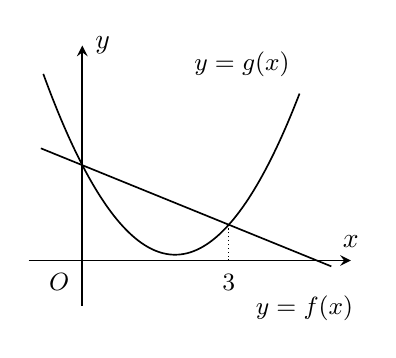
\begin{tikzpicture}[line width=0.6pt, x=0.62cm, y=1.05cm, >=stealth]
  \draw[densely dotted, line width=0.4pt] (3,0) -- (3,0.433);
  \draw[->, line width=0.7pt] (-1.1,0) -- (5.5,0) node[above=1pt] {$x$};
  \draw[->, line width=0.7pt] (0,-0.55) -- (0,2.6) node[right=1pt] {$y$};
  \draw[domain=-0.80:4.45, samples=90, smooth] plot (\x, {0.3*(\x-1.9)^2+0.07});
  \draw[domain=-0.85:5.10] plot (\x, {1.153-0.24*\x});
  \node[anchor=north east, font=\small] at (-0.06,-0.04) {$\pt{O}$};
  \node[anchor=north, font=\small] at (3,-0.05) {$3$};
  \node[anchor=south east, font=\small] at (4.45,2.10) {$y=g(x)$};
  \node[anchor=north, font=\small] at (4.55,-0.30) {$y=f(x)$};
\end{tikzpicture}
